\chapter{sel4}
seL4 fa parte della famiglia dei microkernel L4 che risalgono alla prima metà degli anni '90 creato da Jochen Liedtke per sopperire alle scarse performance dei primi sistemi operativi basati su microkernel, ad oggi fa parte del Trustworthy System.\\
Come descritto poco sopra nell'introduzione, seL4 essendo un microkernel, ha un numero di righe di codice sorgente estremamente piccolo e questo è sufficiente per determinare che non è un sistema operativo ma soltanto un microkernel, infatti non fornisce nessun dei servizi che siamo solitamente abituati a trovare su un comune SO, "è solo un sottile involucro attorno all'hardware" \cite{sel4-whitepaper}, tutti i servizi devono essere eseguiti in modalità utente e questi dovranno essere importati ad esempio da sistemi operativi open-source come Linux (oppure scritti da zero). data questa sua definiamola "incapacità" nel fornire servizi all'utente seL4 è anche un \textit{hypervisor}, quindi è possibile eseguire macchine virtuali sulle quali far girare un comune SO che fornirà i servizi non presenti in seL4.
\begin{figure}[h]
  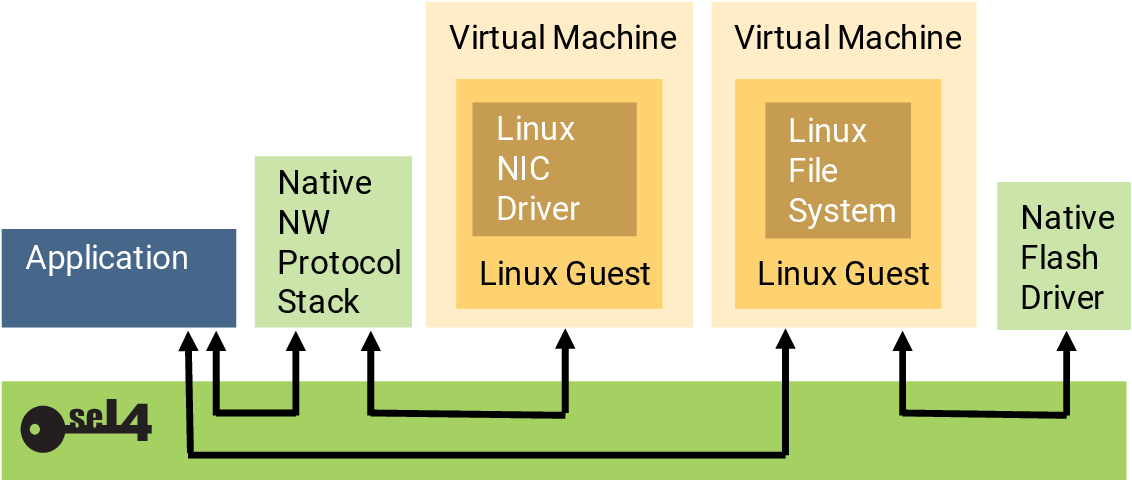
\includegraphics[width=\linewidth]{img/seL4Hypervisor.png}
  \caption{Virtualizzazione del SO Linux per l'intergrazione dei servizi di networking e file system}
  \label{fig:MonolithicVSmicrokernel}
\end{figure}

Un esempio pratico può essere quello mostrato in figura 2, in cui è raffigurato seL4, una generica applicazione e due macchine virtuali (VM) sulle quali viene eseguita una versione ridotta al minimo di Linux, che quindi avrà poco più oltre al servizio che dovrà eseguire.
Queste due VM forniranno all'applicazione il servizio di networking ed il file system per la gestione della memoria secondaria (hard disk, supporti rimovibili ecc.), le comunicazioni tra le parti saranno gestite da un canale fornito dal microkernel ma le due macchine virtuali non avranno modo di comunicare tra di loro, non solo questo ma come si vede in figura anche le comunicazioni tra le varie parti e l'applicazione sono ben delineate e precise, nessun'altra comunicazione tra le varie parti è possibile al di fuori di quelle indicate dalle frecce.

\section{capability}
Una \textit{capability} è definita formalmente come un riferimento ad oggetto, nel nostro caso specifico possiamo definirla anche come un puntatore immutabile, cioè una capability farà sempre riferimento allo stesso oggetto.\\
SeL4 è un sistema capability-based (basato sulle capability) 
questo significa che l'unico modo per eseguire un operazione è attraverso l'invocazione di una capability. Ad ognuna di esse, inoltre, sono associati dei diritti di accesso, quindi una capability è un incapsulamento di un riferimento ad oggetto con i diritti ad esso conferiti.
Per dare una definizione meno formale possiamo pensare alle capability come a delle chiavi di accesso estremamente specifiche riguardo quale entità può accedere ad una particolare risorsa del sistema. Inoltre permettono di supportare il \textit{principle of least privilege}, principio del privilegio minimo chiamato anche \textit{principle of least authority} PoLA, questo principio implica che ogni modulo deve avere accesso solo ed esclusivamente alle risorse strettamente necessarie al suo scopo.
In seL4 quindi i diritti dati ad un componente possono essere ristretti al minimo indispensabile per svolgere il loro lavoro come richiesto dal PoLA e chiaramente questo è un grosso punto a favore per quanto riguarda la sicurezza.\\
Nei sistemi operativi più comuni tipo Windows o Linux l'accesso alle risorse è gestito dalle \textit{access-control list} (ACL), quindi, nel caso specifico di Linux, ad ogni file viene associato un set di bit che determinano quali operazioni (lettura, scrittura, esecuzione) possono essere eseguite su di esso dai vari utenti (proprietario, gruppo, altri) questo però implica che ogni file del sistema con lo stesso set di permessi è a disposizione di quello specifico utente, quindi se ci mettiamo nello scenario di voler avviare un programma, di cui non siamo sicuri della sua attendibilità, su uno specifico file questo non è possibile perchè come può accedere a quel file può accedere anche a tutti gli altri che hanno le stesso ACL.\\
Con le capability questo scenario non si può presentare perchè il kernel consentirebbe un operazione se e solo se chi richiede di eseguire l'operazione ha la "giusta capability" per eseguire l'operazione su quel file. 

\subsection{Proprietà delle capability}
Interposition $\rightarrow$ le capability hanno la proprietà di mettersi in mezzo (interpose) tra chi crea una capability e l'effettivo accesso ad una risorsa: se un utente dà una capability ad un oggetto esso non è in grado di sapere cosa effettivamente sia quell'oggetto, può chiaramente utilizzarlo senza però sapere che tipo di oggetto sia.\\
Delegation $\rightarrow$ le capability supportano la delegazione dei privilegi tra gli utenti: l'utente X ha un oggetto e vuole dare accesso ad esso anche all'utente Y; X può creare una nuova capability e darla ad Y senza conservare nessun riferimento all'utente X che l'ha creata, la nuova capability può anche avere meno diritti di accesso (esempio solo lettura invece di lettura e scrittura) e inoltre X in qualsiasi momento può revocare l'accesso ad Y distruggendo la capability.

\section{Hard Real-Time Systems}
Un \textit{Hard Real-Time System} è un sistema in cui il mancato rispetto di una scadenza può portare al fallimento dell'intero sistema. Un esempio molto alla mano di tutti e semplificato può essere l'autopilot di un'automobile; un veicolo dotato di un software di guida autonoma richiede la presenza di un numero estremamente elevato di sensori esterni ed interni al veicolo e il computer di bordo deve leggere, elaborare e dare una risposta immediata ad ogni minimo cambiamento di un valore proveniente da questi sensori, se ad un certo punto l'elaborazione di un dato richiede più del tempo dovuto, anche solo di qualche millisecondo, c'è il rischio che questo comporti una serie  di ritardi a catena che ad esempio portano al non rilevamento di un oggetto che si sta avvicinando al veicolo, oppure alla mancata correzione della traiettoria e quindi l'abbandono della carreggiata, con conseguenze anche catastrofiche.
$\rightarrow$ Lo scheduling dei processi in seL4 è basato sulla priorità, il kernel di sua iniziativa non cambierà mai la priorità di un processo, è sempre decisa dall'utente.\\
$\rightarrow$ SeL4 quando esegue delle operazioni in modalità kernel queste sono esenti dagli interrupt, all'apparenza questo può sembrare catastrofico se non fosse per il fatto che le chiamate di sistema sono tutte brevi, solo la revocazione di una capability può richiedere tempi più lunghi ma in presenza di queste operazioni seL4 adotta una politica di divisione dell'esecuzione in sotto operazioni più brevi, ed inoltre ognuna di esse può essere annullata e poi ripresa da quel punto in poi, così da poter gestire degli eventuli interrupt in attesa.\\
Questi due punti appena elencati sono requisiti fondamentali per gli Hard Real-Time system, scheduling dei processi basato sulla priorità, che sia quindi facilmente analizzabile, e latenza degli interrupt limitata, essendo gli interrupt disabilitati non ci sarà nessuna latenza dovuta al cambio di contesto per gestire subito l'interrupt e dato che le operazioni sono tutte brevi questo non risulta un problema.
\textcolor{red}{Per seL4 è stata eseguita una worst-case execution time (WCET), questo vuol dire che è stato determinato un limite superiore di latenza di ogni system call nel caso peggiore e ciò implica anche il caso peggiore di latenza di un interrupt}
